\graphicspath{{figures/tower/}}
\chapter{输电塔结构有限元建模}
\section{\SI{500}{kV}南京三江口长江大跨越工程介绍}
\SI{500}{kV}南京三江口长江大跨越工程是山西阳城电厂二期工程电力送出江苏省
内配套等输变电工程的重要组成部分,跨越点在长江南京河段的三江口节点位置。
按耐—直—直—耐实施跨越,档距分布为\SI{520}{m}-\SI{1770}{m}-\SI{520}{m}(图\ref{fig:tower-line}),跨越塔与跨越塔之间的输电线矢高为\SI{132.4}{m},跨越塔与锚塔之间的输电线矢高为\SI{50}{m}。
\begin{figure}[!htbp]
\centering
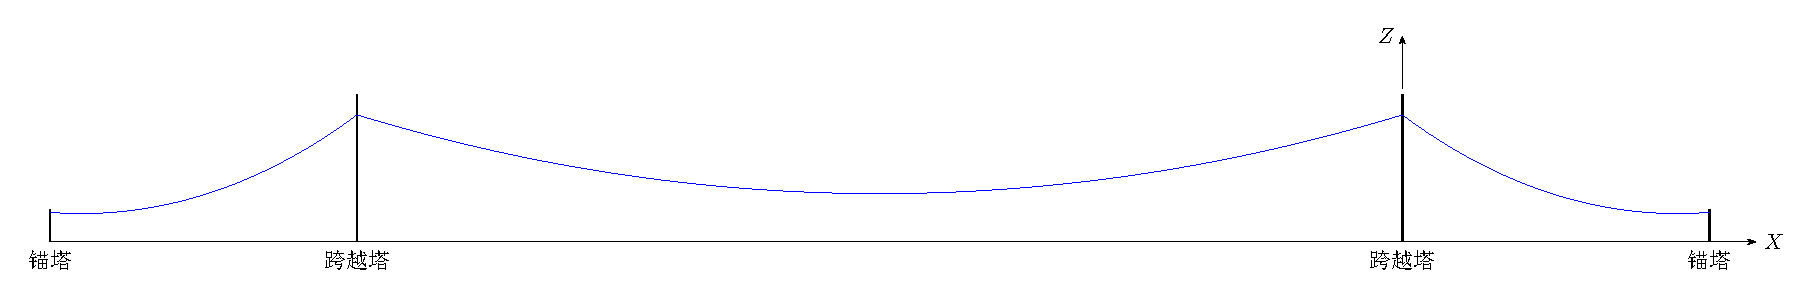
\includegraphics[width=\textwidth]{tower_line_system.pdf}
\caption{三江口大跨越示意图}
\label{fig:tower-line}
\end{figure}

大跨越南、北跨越塔均为双回路蝶型布置的钢管塔,呼高\SI{215}{m},全高\SI{249.5}{m},根开\SI{49.6}{m},单基塔重(含旋梯及走道)共\SI{1924}{t}。
钢管塔最大管径\SI{1480}{mm},相应壁厚\SI{25}{mm},钢管材质采用Q345B和Q235B级钢,最大螺栓直径\SI{56}{mm},螺栓采用6.8级和8.8级两种。
大跨越输电塔(下文简称大跨越塔)实物如图\ref{fig:real-tower}所示。
锚塔为单回干字型角钢塔,锚塔横担垂直于跨越段中心线布置,根开为\SI{16}{m}$\times$\SI{24}{m}布置,呼高\SI{24}{m},全高\SI{55}{m},单基塔重\SI{106}{t}。
每个回路分别对应2基铁塔,共使用4基锚塔。

导线采用四分裂布置,型号为 AACSR/EST-500 特强钢芯铝合金绞线,两根地线采用 36芯的OPGW-325型复合光缆,光缆为层绞结构。
导线、OPGW均为整根,跨越耐张段没有接头。锚塔上跳线采用LGJ-630/45型钢芯铝绞线,越侧耐张绝缘子串引流线夹与LGJ-630/45型钢芯铝绞线匹配。跨越塔导线采用四联530k N级盘瓷悬垂绝缘子串,OPGW采用双联预绞式悬垂金具串;锚塔导线采用六联400k N级盘瓷耐张绝缘子串,OPGW采用预绞式耐张金具串。
\begin{figure}[!htbp]
\centering
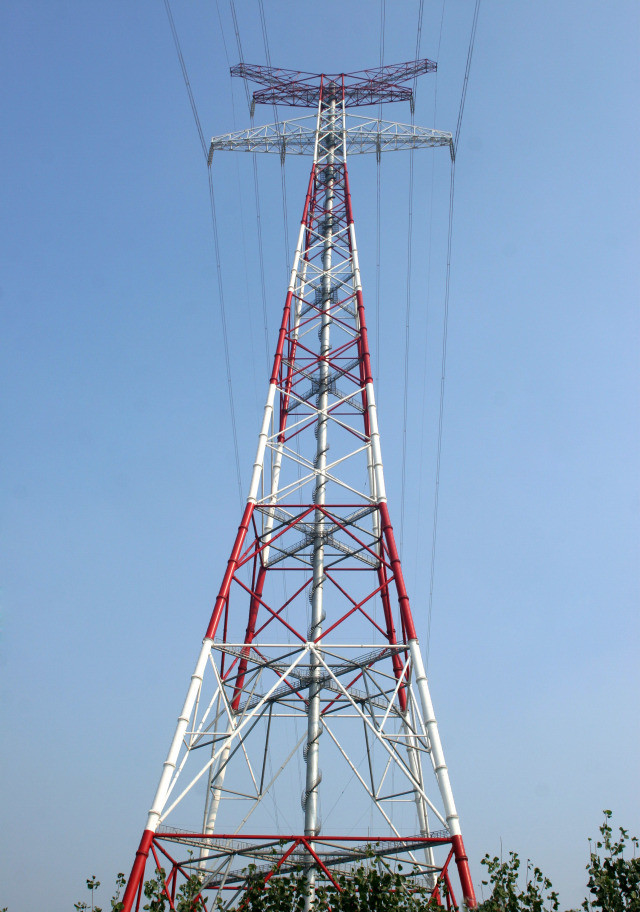
\includegraphics[width=\textwidth]{tower.png}
\caption{三江口大跨越输电塔}
\label{fig:real-tower}
\end{figure}

\section{输电塔有限元模型}
本文选择大型通用有限元软件ANSYS Mechanical APDL进行输电塔建模。

\subsection{输电塔塔体模拟}\label{sec:tower-fea}
选用二节点非线性三维梁单元BEAM 188模拟输电塔构件。
单元每个节点处包括三个平动自由度和三个转动自由度。
输电塔构件之间为多孔螺栓连接,有限元模型以刚性节点模拟。
输电塔的有限元模型见\ref{fig:tower-fea}所示。
考虑到输电塔为空间对称结构,取塔的底面中心为坐标原点,高度方向为$Z$轴方向,输电线方向为$X$轴方向(图\ref{fig:tower-line}、\ref{fig:tower-fea})。
\begin{figure}[!htbp]
\centering
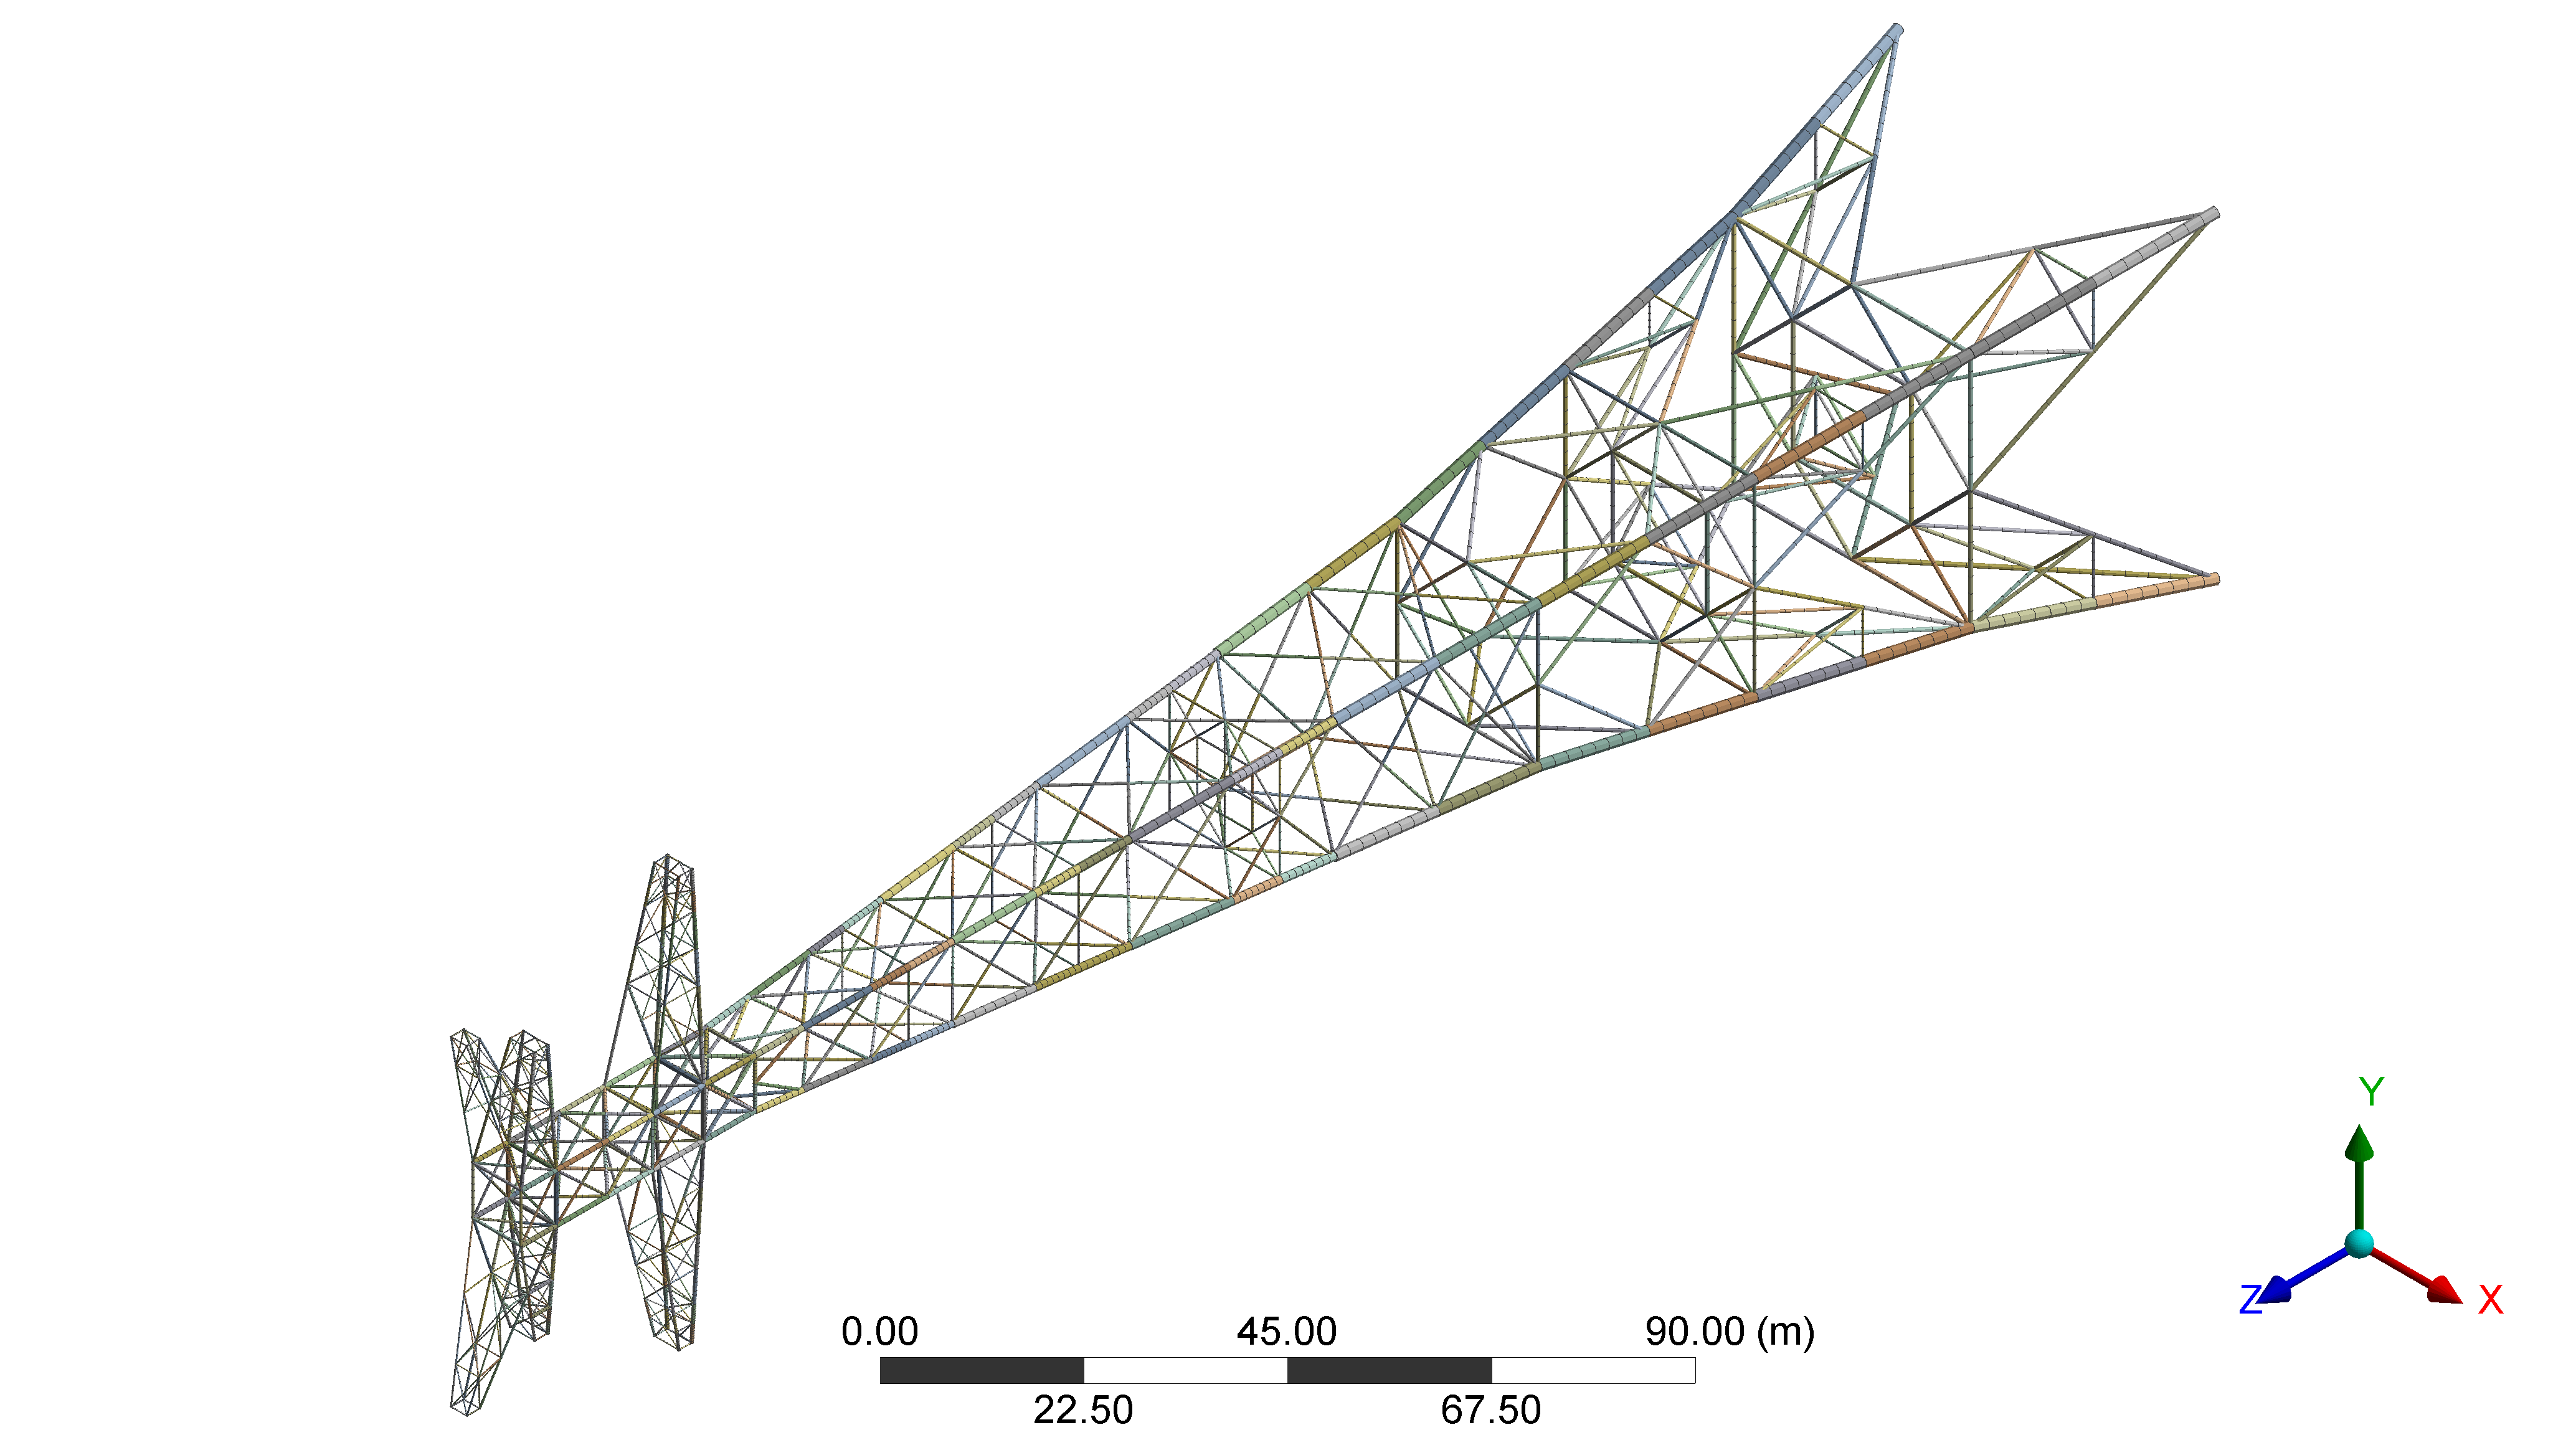
\includegraphics[width=\textwidth]{tower_fea.png}
\caption{输电塔有限元模型}
\label{fig:tower-fea}
\end{figure}

\subsection{输电导线模拟}


\section{输电塔结构模态分析}
